The PyCBC Live early warning search identifies \gwadj signals prior to merger, giving warning to the international astronomy community of an incoming \gwadj event. The early warning search is an adaptation to the PyCBC Live full bandwidth search---discussed heavily in chapter~\ref{chapter:5-pycbc-live}---and we have identified problems relating to search for pre-merger signals which require changes to be made to the early warning infrastructure to improve the sensitivity of the pipeline.

In Section~\ref{6:sec:multi-messenger-astronomy} we discuss the joint detection of astrophysical events with both \gw and electromagnetic observatories, in Section~\ref{6:sec:gw170817} we highlight the only multi-messenger event seen thus far and the timeline of observations. The PyCBC Live early warning search is described in Section~\ref{6:sec:early-warning-search} with the template bank construction in Section~\ref{6:sec:early-warning-template-bank} and how sky localisation for events is obtained in Section~\ref{6:sec:event-localisation}. Section~\ref{6:sec:gw170817-in-ew} uses GW1701817 as an example to demonstrate the capabilities of the early warning search and in Section~\ref{6:sec:injection-tests} we describe a full injection set test performed using the early warning search to identify any problems and the results of this search. Finally, in sections~\ref{6:sec:false-problems} and~\ref{6:sec:missing-cands} we discuss the problems found when testing the early warning search, the cause of the problems and the potential solutions to these problems.

\section{\label{6:sec:multi-messenger-astronomy}Multi-messenger astronomy}

The PyCBC \gwadj search pipeline searches for \gwadj signals from the merger of two compact objects~\cite{PyCBC:2016}. Black holes do not emit electromagnetic radiation and therefore the merger of two black holes can currently only be directly observed with \gwadj detectors~\cite{Ghez:2000}. Neutron stars, on the other hand, are electromagnetically bright themselves and the merger of two neutron stars might produce a kilonova~\cite{Kilonovae:2017}. Kilonovae emit a broad range of electromagnetic radiation across the spectrum~\cite{kilonova_lightcurve:2017} which can be observed with many of the ground and space-based electromagnetic observatories we have on Earth. The combination of \gw and electromagnetic emissions allows us to understand more about these events than either observation could provide alone~\cite{multi_mess_astro:2019}. Astrophysical events which have been observed with more than one type of signal are called multi-messenger events, this can be from any of the three: electromagnetic signals, \gws or neutrinos. We will use the term `multi-messenger event' to describe an event which has been seen with a \gwadj signal and an electromagnetic counterpart.

One such quantity that can be measured from observing kilonovae with both \gws and electromagnetic radiation is the Hubble constant~\cite{Schutz:1986}, the measured rate of expansion of the Universe~\cite{hubble:1929}. The Hubble constant is currently determined across two distance scales using purely electromagnetic observations: firstly, the large scale cosmological measurements using the cosmic microwave background~\cite{WMAP_H0:2003} and baryon acoustic oscillations~\cite{BAO_H0:2009} and secondly, the local Universe scale using the astrophysical standard candle Cepheid variable stars~\cite{Cepheids_H0:2001} and type Ia supernovae~\cite{TypeIa_H0:1998}. The Hubble constant values obtained at the different scales do not agree~\cite{H0_tension:2020} so by combining the observation of binary neutron star signals using both \gw and electromagnetic observatories we can provide an independent measurement of the Hubble constant to break this tension.

At nearby distances ($d \lesssim 50 \, \text{Mpc}$) the Hubble constant can be calculated using Hubble's law~\cite{hubble:1929},
%
\begin{equation}
    v = H_{0} d,
    \label{6:eq:basic_hubbles_law}
\end{equation}
%
where $v$ is the recessional velocity of a source, $H_{0}$ is the Hubble constant and $d$ is the proper distance to the source. For nearby objects ($z \lesssim 0.1$): $v$ can be approximated as $v \approx cz$, where $z$ is the redshift of the object and $c$ is the speed of light; luminosity distance is approximately equal to the proper distance $d \approx D_{L}$. On small distance scales the expansion of the universe doesn't greatly affect these measurements. We obtain an equation for the Hubble constant at short distances
%
\begin{equation}
    H_{0} = c \frac{z}{D_{L}}.
    \label{6:eq:hubbles-law}
\end{equation}
%

The expansion rate of the Universe historically is not constant. For objects at larger distances we have to account for redshift in the luminosity distance. We begin by defining the luminosity distance in terms of the comoving distance,
%
\begin{equation}
    D_{L}(z) = (1 + z)D_{c}(z),
\end{equation}
%
which accounts for the expanding universe in the term $(1 + z)$. The comoving distance is given by
%
\begin{equation}
    D_{c}(z) = c \int^{z}_{0} \frac{dz^{\prime}}{H(z^{\prime})},
\end{equation}
%
where the Hubble constant, $H(z^{\prime})$, is now the Hubble parameter at redshift $z^{\prime}$ and depends on the model of cosmology.
We can use the comoving distance to get an expression for the luminosity distance,
%
\begin{equation}
    D_{L}(z) = (1 + z) c \int^{z}_{0} \frac{dz^{\prime}}{H(z^{\prime})}.
\end{equation}
%
$H_{0}$ will depend on the cosmological parameters representing the density of matter, radiation and dark energy. To measure the Hubble constant we need to measure the redshift and luminosity distance of multiple sources.

The luminosity distance of a \gwadj event is inversely proportional to the amplitude of the \gwadj strain~\cite{Schutz:1986},%
\begin{equation}
    h(t) \propto \frac{1}{D_{L}} , 
\end{equation}
%
which is obtained via \gwadj searches and parameter estimation. The \gwadj strain amplitude does have a degeneracy with the inclination angle, $\iota$, of the binary neutron star system which is described as the angle between the line of sight to the observer and the orbital angular momentum of the source~\cite{inclin_degen_2:2019}.

The \gwadj strain dependence on inclination angle manifests differently in the two \gwadj polarisations and can be simply described as~\cite{inclin_degen:2018},
%
\begin{align}
    h_{+} &\propto \left(1+\cos^{2}\iota\right), \\
    h_{\times} &\propto \cos\iota .
    \label{6:eqn:inclin_polarisations}
\end{align}
%
It can be seen from Equation~\ref{6:eqn:inclin_polarisations} that an edge-on system ($\iota = 90^{\circ}$) will produce a signal entirely in the $h_{+}$ polarisation but a face-on system will produce a mixed signal with contributions from both $h_{+}$ and $h_{\times}$. The inclination angle degeneracy could be broken if we were able to measure $h_{+}$ and $h_{\times}$ independently, but the individual \gwadj detectors are sensitive only to a linear combination of the polarisations~\cite{aLIGO:2015}. Multiple \gwadj detectors with different orientations will be sensitive to different linear combinations of $h_{+}$ and $h_{\times}$ and are therefore required to break this degeneracy and fully reconstruct the source orientation~\cite{inclin_degen_2:2019}.

The redshift of a \gwadj event is embedded in the \gwadj signal via the chirp rate of the system. The chirp rate is defined as the rate of change of the \gwadj frequency and is given to leading order as~\cite{Jaranowski:2009}
%
\begin{equation}
    \frac{df}{dt} = \frac{96}{5} \pi^{8/3} \left(\frac{G\mathcal{M}}{c^{3}}\right)^{5/3} f^{11/3}.
    \label{6:eq:chirp_rate}
\end{equation}
%
The rate of change of the \gwadj frequency is easy to measure and will give us the chirp mass of the system,
%
\begin{equation}
    \mathcal{M} = \frac{(m_1 m_2)^{\frac{3}{5}}}{(m_1 + m_2)^{\frac{1}{5}}}.
    \label{6:eq:mchirp}
\end{equation}
%
which depends on the two masses of the system, $m_{1}$ and $m_{2}$. The observed $\mathcal{M}$ is redshift dependent,
%
\begin{equation}
    \mathcal{M}_{obs} = \mathcal{M}_{source}(1 + z), 
    \label{6:eq:mchirp_obs}
\end{equation}
%
and $\mathcal{M}_{obs}$ is scaled by the redshift where events with larger redshifts will appear with larger observed chirp masses than their source chirp mass, $\mathcal{M}_{source}$. We would require a measurement of the Hubble constant to determine the redshift using the luminosity distance and we reach a circular argument.

We can look at other ways to measure the redshift of the event without using the \gwadj signal. The primary candidate is an electromagnetic emission from the event, for example, a kilonova from a binary neutron star system. Using the electromagnetic emission we can locate the host galaxy of the source and find the approximate redshift of the binary neutron star system. We will then have a luminosity distance, measured by the \gwadj signal, and a redshift, measured by the electromagnetic observation, and using Equation~\ref{6:eq:hubbles-law} we can calculate the Hubble constant. This combination of event information from two separate sources of information for the same event means we can use electromagnetically bright \gwadj sources as another standard siren for measuring the Hubble constant, highlighting the importance of observing multi-messenger events.

\section{\label{6:sec:gw170817}GW170817: The only multi-messenger event so far}

We have described multi-messenger events as those that have been seen with a \gw and an electromagnetic signal, in reality the event will broadcast information across the electromagnetic spectrum at varying timescales so we might see a single \gwadj signal but multiple electromagnetic signals. There are observatories around the globe and in space which span this entire spectrum and can observe counterparts to our \gwadj signal in all the different frequency ranges: from high frequency gamma rays to long wavelength radio waves. 

GW170817~\cite{GW170817:2017} is the first and only multi-messenger event we have observed, the Q-scans depicting the \gwadj signal found by the three detectors online at the time of the event can be seen in Figure~\ref{6:fig:gw170817_qscan} and the GCN circular~\cite{gcn_circulars:2024} (rapid astronomical bulletins submitted by and distributed to the global physics community) can be found at: \href{https://gcn.gsfc.nasa.gov/other/G298048.gcn3}{https://gcn.gsfc.nasa.gov/other/G298048.gcn3}. On the 17th August 2017 at precisely 12:41:04 UTC, the \gws from the merger of a binary neutron star system were seen by LVK detectors. Only $1.7$ seconds later, a gamma-ray burst (GRB 170817A~\cite{gw170817_joint:2017}) was seen by Fermi~\cite{Fermi:2022, Fermi_GW170817:2017} and INTEGRAL~\cite{INTEGRAL:2003, INTEGRAL_GW170817:2017}. The kilonova emissions were seen next, visual light by the Hubble Space Telescope (HST)~\cite{HST:2000, HST_GW170817:2021} at 11 hours, infrared by HST, VISTA~\cite{VISTA:2015, VISTA_GW170817:2017} and Spitzer~\cite{Spitzer:2004, Spitzer_GW170817:2018} at 12 hours and UV by Swift's UVOT~\cite{Swift:2004, Swift_GW170817:2017} at 15.3 hours post-merger. The final electromagnetic frequencies to be seen were X-rays by Chandra~\cite{Chandra_GW170817:2017} at 9 days post-merger and radio waves by VLA~\cite{VLA:2019, VLA_GW170817:2017} at 16 days post-merger.
%
\begin{figure}
    \centering
    \includegraphics[width=0.8\linewidth]{images/6_earlywarning/gw170817/GW170817_qscan.pdf}
    \caption{The three detector (LIGO-Hanford (top), LIGO-Livingston (middle) and Virgo (bottom)) time-frequency images (Q-scan~\cite{qscan:2004} showing data containing the first binary neutron star \gwadj event, GW170817~\cite{GW170817:2017}, with times shown relative to 17th August 2017 12:41:04 UTC. The detector amplitudes are individually normalised for that detector's amplitude spectral density. The glitch observed in the LIGO-Livingston detector has been subtracted, the technique and results when doing so are presented in section IV of~\cite{GW170817:2017} and this figure is taken directly from figure 1 in~\cite{GW170817:2017}.}
    \label{6:fig:gw170817_qscan}
\end{figure}
%

Analysing GW170817's \gwadj signal and electromagnetic emissions reveal a binary neutron star system located in the Hydra constellation belonging to the galaxy NGC 4993~\cite{NGC4993:1998}. Using these signals the Hubble constant can be inferred as $H_0 = 70.0^{+12.0}_{-8.0} \, \text{km} \, \text{s}^{-1} \,\text{Mpc}^{-1}$~\cite{GW170817_H0:2017} which is consistent with both the measured cosmological value for $H_0$ ($67.74 \pm0.46 \, \text{km} \, \text{s}^{-1} \,\text{Mpc}^{-1}$~\cite{Planck_H0:2015}) and the astrophysical value for $H_0$ ($73.24 \pm1.74 \, \text{km} \, \text{s}^{-1} \,\text{Mpc}^{-1}$~\cite{Riess_H0:2016}) but, it is not accurate enough to break the tension between both values. To constrain the value of the Hubble constant further, we need to observe many more electromagnetically bright events~\cite{Palmese:2021}. Using GW170817 we were able to determine other physical properties such as the speed of gravity~\cite{Harry_speed_of_gravity:2022, Baker_speed_of_gravity:2022}.

Using the electromagnetically bright multi-messenger events to constrain the measurement of the Hubble constant is straight forward. We are also able to use `dark siren' events, which have no electromagnetic counterpart and so rely entirely on the \gwadj emission to measure the redshift. To identify the redshift of dark sirens must use galaxy catalogues and \gwadj sky maps to locate the host galaxy of the \gwadj signal. This is not discussed further in this chapter, for more information on dark sirens please look to~\cite{DES:2019, Dalang_dark_sirens:2023}

\section{\label{6:sec:early-warning-search}Detecting \gwadj events pre-merger}

\Gwadj signals from low-mass sources merge at frequencies above the sensitive frequency band of the LIGO \gwadj detectors~\cite{aLIGO_design_curve:2018}. The lower sensitive frequency of the LIGO detectors is ${\sim}20 \, \text{Hz}$ meaning the \gwadj signal can exist in the sensitive band for potentially hundreds of seconds before it is identified by the \gwadj search pipelines. Figure~\ref{6:fig:snr_accumulation} shows the accumulation of SNR over a $1.4 \, \text{M}_{\odot}{\text{--}}1.4 \, \text{M}_{\odot}$ binary neutron star signal; at $29 \, \text{Hz}$, 
$31 \, \text{\%}$ of the SNR is accumulated at $83 \, \text{Hz}$ of the total template duration.
%
\begin{figure}
    \centering
    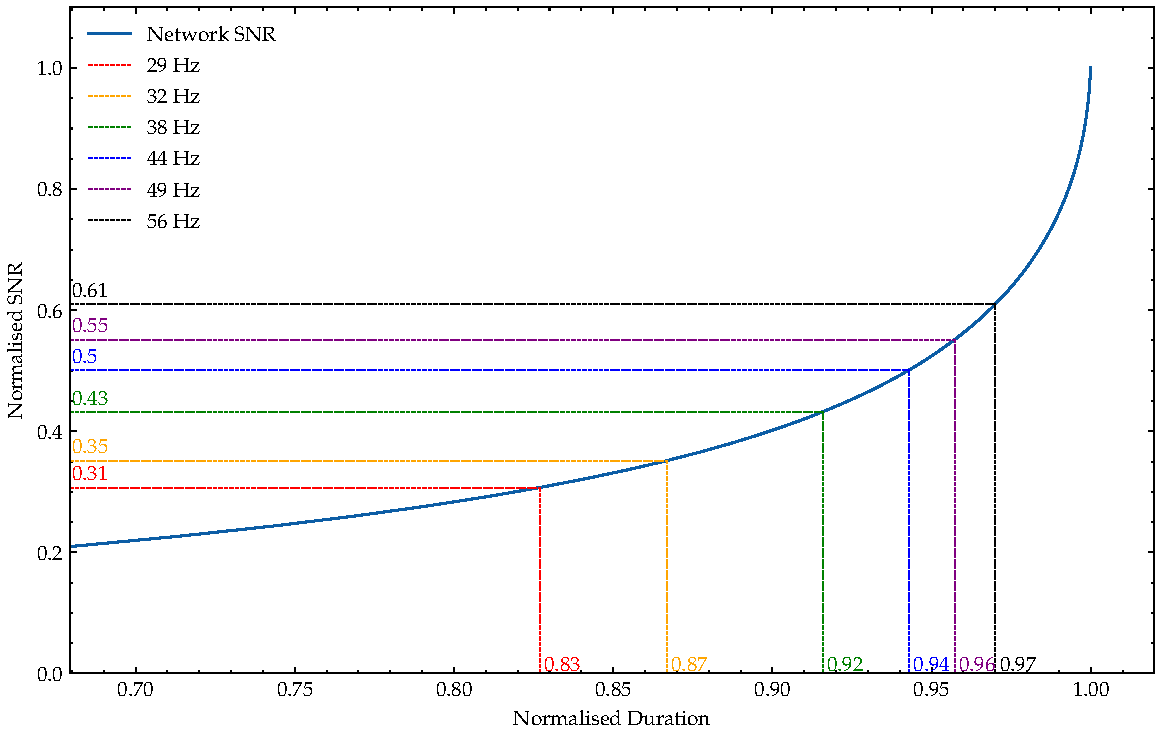
\includegraphics[width=1.0\linewidth]{images/6_earlywarning/snr_accumulation.pdf}
    \caption{The accumulation of signal-to-noise ratio over the duration of a $1.4 \, \text{M}_{\odot}{\text{--}}1.4 \, \text{M}_{\odot}$ binary neutron star system. SNR and duration have been normalised such that the SNR and duration at an initial signal frequency of $15 \, \text{Hz}$ and a final signal frequency of $1024 \, \text{Hz}$ is equal to $1$.}
    \label{6:fig:snr_accumulation}
\end{figure}
%

This presents an opportunity to detect the \gwadj signal before it merges, in the inspiral regime of the system. The visible electromagnetic counterpart to the \gwadj signal is produced post-merger, therefore, by disseminating information about an ongoing \gwadj event prior to the merger we are able to give enough warning to electromagnetic observatories to slew their telescopes to the approximate region on the sky in which we will indicate a \gwadj event will occur. Providing this warning pre-merger is commonly referred to as `early warning'. This section details the methodologies used in the PyCBC Live early warning search to achieve the detection of electromagnetically bright \gwadj signals pre-merger.

Even with an accurate sky map and dedicated electromagnetic telescopes (for example, GOTO is used for \gwadj event follow-up~\cite{GOTO:2020}), the gamma-ray burst counterparts can arrive less than two seconds after merger, not giving us enough time to identify the signal, produce a sky map and slew any telescopes to the correct sky location.

\subsection{\label{6:sec:pycbc-ew-search}The PyCBC Live early warning search}

% What has been scaled back
To identify potential \gwadj signals prior to the merger of the compact objects, the PyCBC Live search pipeline has created an optimised early warning search for pre-merger gravitational waveforms. In this section, we describe the design choices which allow the early warning search to operate in the early warning regime.

We use two terms when referring to search detection times: latency refers to the time taken by the search to identify a \gwadj template and produce a \gwadj event; warning refers to the time prior to the \gwadj signal's merger that the event was identified. The early warning attempts to maximise the warning time, which is improved by decreasing the latency between detection and event production.

% What has been optimized
We can divide the latency of detection into three contributing components: firstly, the analysis stride of the early warning search is one second, therefore a signal will have to wait until the entire second has arrived before it can be processed; secondly, when highpassing and overwhitening\footnote{Dividing the data by the PSD~\cite{FINDCHIRP:2012}.} our data we introduce corruption to the edge samples, we pad the data by an extra $1.5 \, \text{seconds}$ to account for this, which the signal has to wait for; thirdly, we need to analyse the data to detect the signal, we impose a strict analysis time requirement of less than the analysis stride, so data does not build up in the processing queue. In total, we have a minimum latency of $2.5 \, \text{seconds}$ (if the signal appears in the final few samples of the analysis stride) and a maximum latency of $3.5 \, \text{seconds}$ (if the signal appears in the first few samples of the analysis stride). Figure~\ref{6:fig:latency_plot} shows minimum and maximum latencies of both the full bandwidth and early warning search.
%
\begin{landscape}
\begin{figure}
    \centering
    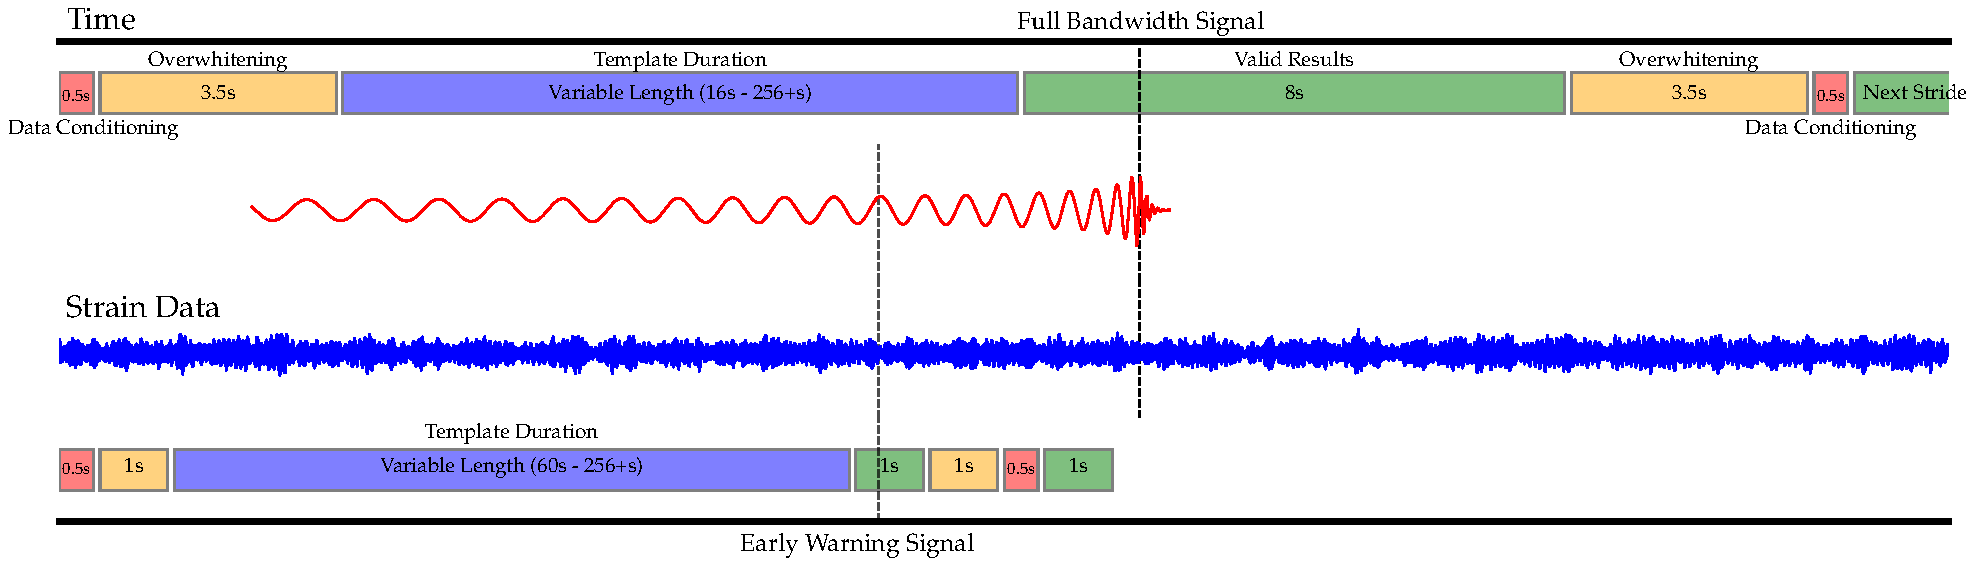
\includegraphics[width=\columnwidth]{images/6_earlywarning/gw170817/latency_plot_new_font.pdf}
    \caption{An illustration of the detection latency between template end and event upload to GraceDB~\cite{ligo_gracedb:2024}. The top half of the plot pertains to the PyCBC Live Full Bandwidth search and indicates that the search has a maximum latency of $20$ seconds, the bottom half describes the PyCBC Live Early Warning search which has a maximum latency of $3.5$ seconds. From the end of the \gwadj template the search must wait for the current analysis stride to end, another period of data must then be waited on (overwhitening and data conditioning) and then the search analyses the previous analysis stride during the next analysis stride.}
    \label{6:fig:latency_plot}
\end{figure}
\end{landscape}
%
By comparison, the full bandwidth search has a minimum and maximum latency of $12$ to $20$ seconds respectively, with no possibility to observe the event pre-merger.

% How does it do it
To ensure the processing time for the triggers is completed in less than one second aspects of the search have been simplified: we search over only two interferometers (LIGO-Hanford and LIGO-Livingston) and we use a simple new SNR single detector ranking statistic and phase-time-amplitude histogram coincident ranking statistic. Alongside this, the early warning search has a far smaller template bank of only $9180$ templates compared to the ${\sim}700,000$ templates in the full bandwidth template bank.

\subsection{\label{6:sec:early-warning-template-bank}Frequency truncated template bank}

The template bank used by the PyCBC Live early warning search is composed of frequency truncated templates. These are \gwadj templates which start at a lower frequency and end in the inspiral phase at a upper frequency cutoff. The bank contains six different frequency cutoffs at: $29$, $32$, $38$, $44$, $49$ and $56 \, \text{Hz}$. These frequencies correspond to approximately $60$, $46$, $29$, $20$, $15$ and $10$ seconds before merger for a $1.4 \, \text{M$_\odot$}$\text{--}$1.4\, \text{M$_\odot$}$ binary neutron star signal.

The PyCBC Live early warning template bank is constructed by generating six separate template banks (one for each frequency cutoff) using a geometric placement algorithm~\cite{Harry_Lundgren:2012} with a minimal match between templates of $0.97$. The template parameters of the bank are chosen to represent potentially electromagnetically bright signals, these are produced by the merger of low mass binary neutron star or neutron star black hole systems. The masses of the two compact objects is limited between $1\text{--}3 \, \text{M$_\odot$}$ and to reduce the size and complexity of the template bank we use zero-spin on both components. The PSD used to generate the template bank is representative of the Advanced LIGO design curve that includes estimates for the main fundamental noises of the interferometer, in particular: seismic noise, thermal noise and quantum noise~\cite{aLIGO_design_curve:2018} with a binary neutron star range of $140 \, \text{Mpc}$~\cite{ligo_prospects:2016}. The six early warning template banks combined contain $9180$ templates.
%
\begin{figure}
    \centering
    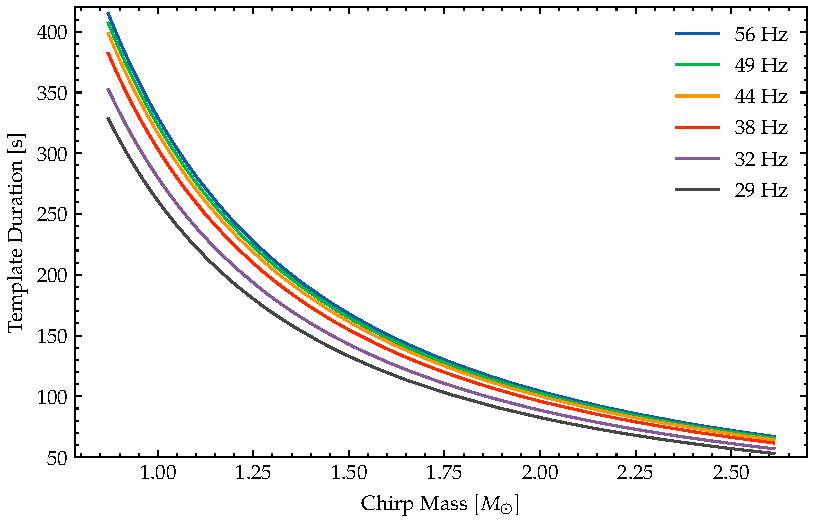
\includegraphics[width=\textwidth]{images/6_earlywarning/search/template_bank_duration_mchirp.pdf}
    \caption{Template duration versus chirp mass, $\mathcal{M}$, for different frequency cutoffs in the early warning template bank. Each curve corresponding to a different frequency cutoff, $f_{final}$, ($29\text{--}56  \, \text{Hz}$). The chirp mass is calculated from the component masses of the binary system, and the template duration is calculated between the lower frequency, $17 \, \text{Hz}$ and the frequency cutoff, $f_{final} \, \text{Hz}$.}
    \label{6:fig:tb_duration_mchirp}
\end{figure}
%
The duration of templates at each final frequency cutoff can be seen in Figure~\ref{6:fig:tb_duration_mchirp} as a function of the chirp mass, $\mathcal{M}$, of the template. It can be seen that higher $\mathcal{M}$ templates have shorter duration and templates with a lower frequency cutoff also have shorter duration when compared to templates with the same $\mathcal{M}$ but a higher frequency cutoff.

\subsection{\label{6:sec:event-localisation}Determining event sky locations}

% (BRILLIANT PAGE FOR THIS https://emfollow.docs.ligo.org/userguide/early\_warning.html)

We call a \gwadj candidate obtained by the early warning search an `event'. These events have information about the \gwadj parameters and make a prediction of the time of coalescence of the \gwadj signal. Identifying the sky location of the event is critical for multi-messenger astronomy. With a sky location, the \gwadj observatories are able to tell electromagnetic observatories where to slew their telescopes to see the event prior to merger, to have the best chance of seeing electromagnetic counterparts as possible.

We describe the sky location with three parameters: right ascension, declination, and distance. Distance is measured from the \gwadj signal, as previously described and we  measure the right ascension and declination using two key pieces of information: the time difference between time of arrivals at different detectors which allows us to calculate a time-of-arrival triangulation; and amplitude differences between the signal strength measured by each detector to determine the \gwadj polarisation, the individual detector quadrupolar sensitivity pattern of the antenna response will favour particular sky locations where the detector is more sensitive to \gws coming from certain angles. The greater number of \gwadj detectors in the network lead to more accurate sky location triangulation. Figure~\ref{6:fig:gw170817_skymap} shows the sky map created for GW170817~\cite{gw170817_skymap:2017} with the source location identified by the LIGO-Hanford and LIGO-Livingston detectors shown in the green dashed contour (representing the 90\% confidence interval).
%
\begin{figure}
    \centering
    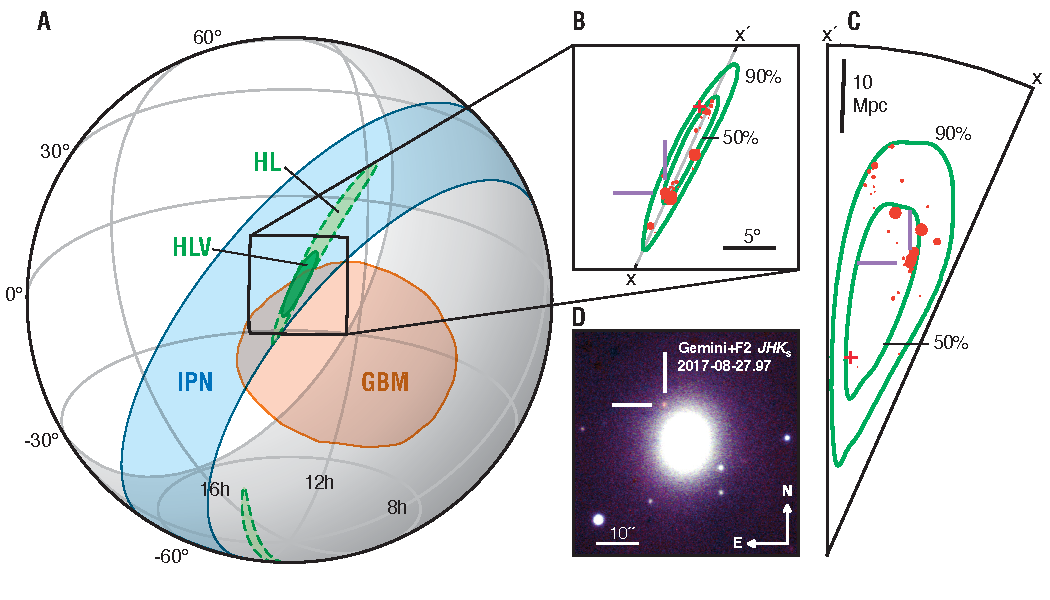
\includegraphics[width=1.0\linewidth]{images/6_earlywarning/gw170817/GW170817_skymap.pdf}
    \caption{The localisation of GW170817 and associated electromagnetic counterpart. The rapid LIGO localisation is indicated by the green dashed contour, and the LIGO \& Virgo localisation by solid green. Fermi~\cite{Fermi:2022} is shown in orange, and the Interplanetary Network triangulation from Fermi and INTEGRAL~\cite{INTEGRAL:2003} in blue. This figure is taken directly from~\cite{gw170817_skymap:2017}}
    \label{6:fig:gw170817_skymap}
\end{figure}
%

A greater number of detectors observing the event will produce more accurate sky locations; adding a third detector to the network (like Virgo~\cite{aVirgo:2015}) is required for a point sky location. BAYESTAR~\cite{BAYESTAR:2016} is a tool for providing accurate sky maps from \gwadj events in as little as a few seconds. As a \gwadj signal is observed by templates with higher and higher frequency cutoffs, the sky map will become more accurate due to the increase in accumulated SNR. To demonstrate the improving sky map localisation as the signal progresses through our template bank we can produce the sky maps found by the early warning search when looking for a $1.4 \, \text{M$_\odot$}\text{--}1.4 \, \text{M$_\odot$}$ binary neutron star injection at a random point on the sky. The \gwadj injection is placed at a distance such that the full bandwidth SNR of the signal is $30$. Figure~\ref{6:fig:ew_30SNR_multiple} shows the sky map displaying the 90\% confidence interval contours for every frequency cutoff in the template bank as well as the full bandwidth sky map, the sky location of the injection can be seen as a star on the sky map. In the legend of the figure, you can see the decreasing sky localisation area as frequency cutoff increases.
%
\begin{figure}
    \centering
    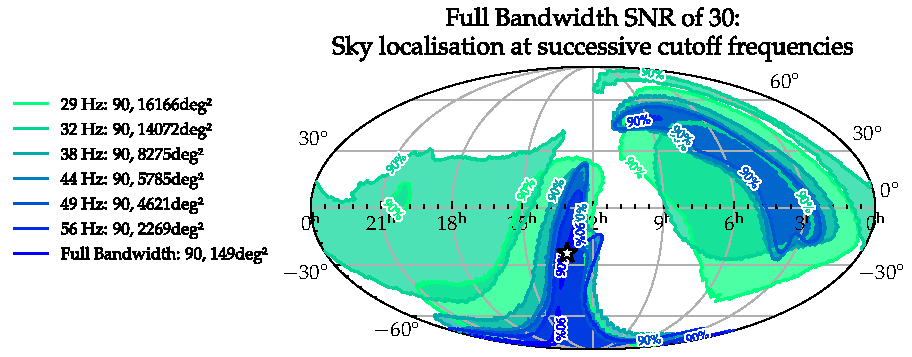
\includegraphics[width=\textwidth]{images/6_earlywarning/localisation/30SNR_multiple.pdf}
    \caption{The \gwadj sky localisation probability map (sky map) corresponding to a $1.4 \, \text{M$_\odot$}\text{--}1.4 \, \text{M$_\odot$}$ binary neutron star signal with a full-bandwidth (upper frequency cutoff $= 1024 \, \text{Hz}$) signal-to-noise ratio of $30$. The successive $90\%$ confidence interval sky map contours for frequency cutoffs from $29\text{--}56 \, \text{Hz}$ are shown, where it can be seen that a higher frequency cutoff leads to a more accurate sky map.}
    \label{6:fig:ew_30SNR_multiple}
\end{figure}
%
\begin{table}[ht]
    \centering
    \setlength{\tabcolsep}{4pt}
    \rowcolors{4}{white}{lightgray}
    \begin{tabular}{cccc}
        \toprule
        \textbf{Full SNR} & \textbf{10} & \textbf{20} & \textbf{30 (Fig.~\ref{6:fig:ew_30SNR_multiple})} \\
        \midrule
        \textbf{Frequency [Hz]} & \multicolumn{3}{c}{\textbf{Localisation area [deg$^{2}$] (90\% credible area) }} \\
        \cmidrule(lr){2-4}
        29 & Not Found & 26,583 & 16,166 \\
        32 & Not Found & 22,464 & 14,072 \\
        38 & Not Found & 12,303 & 8,275 \\
        44 & 18,584 & 8,408 & 5,785 \\
        49 & 14,068 & 6,758 & 4,621 \\
        56 & 9,636 & 4,679 & 2,269 \\
        1024 & 1,908 & 300 & 149 \\
        \bottomrule
    \end{tabular}
    \caption{The sky localisation areas found by BAYESTAR~\cite{BAYESTAR:2016} for three different \gwadj injections injected at the same sky location but with different distances so as their full bandwidth signal-to-noise ratio to be equal to the `Full SNR'. The sky localisation 90\% confidence interval is shown for the six frequency cutoffs found in the PyCBC Live early warning template bank~\cite{PyCBC_earlywarning:2020} as well as the sky localisation area for the full bandwidth ($1024 \, \text{Hz}$) event. Events which weren't found above the PyCBC Live early warning search signal-to-noise ratio threshold for a frequency cutoff have no sky localisation and have been given a value of `Not Found' in the table.}
    \label{6:tab:skymap_early_warning}
\end{table}
%

We can do the same for an injection placed at a distance such that the full bandwidth SNR is $10$ and $20$ and display the sky localisation areas at the different frequency cutoffs in Table~\ref{6:tab:skymap_early_warning}. The $10$ SNR injection was not seen by the early warning search for frequency cutoffs $29$ and $32 \, \text{Hz}$, this is due to an event not being found above the search's SNR threshold. It is clear that a larger frequency cutoff leads to a more accurate sky localisation.

\section{\label{6:sec:gw170817-in-ew}Detecting GW170817 in early warning}

GRB 170817A was seen by Fermi $1.7$ seconds after GW170817 was seen by LVK. Fermi observes the complete sky over a ${\sim}90 \, \text{minute}$ period~\cite{Fermi:2022} and can enter a pointing mode to re-point toward high profile events, such as those reported by \gwadj detectors. With the GRB counterpart being the earliest confirmation of a multi-messenger event, it is even more important that \gwadj observatories provide as much warning for an event to allow other telescopes to be in position for detecting electromagnetic counterparts. The \gwadj signal from GW170817 could have been detected by a $29 \, \text{Hz}$ template $67$ seconds pre-merger, that is $67$ seconds warning we can provide to electromagnetic observatories.

GW170817 was seen by \gwadj searches and the initial GCN circular was distributed $27$ minutes after merger time. The LIGO-Livingston data contained a very loud glitch which had to be removed before a sky map could be made, leading to a sky map latency of $5$ hours and $14$ minutes. The Q-scan containing the glitch can be seen in Figure~\ref{6:fig:gw170817_glitch}~\cite{GW170817:2017}. The original event was uploaded to GraceDB (the Gravitational Wave Candidate Event Database~\cite{ligo_gracedb:2024}) and can be seen at on this web page: \href{https://gracedb.ligo.org/events/G298048}{https://gracedb.ligo.org/events/G298048}.
%
\begin{figure}
    \centering
    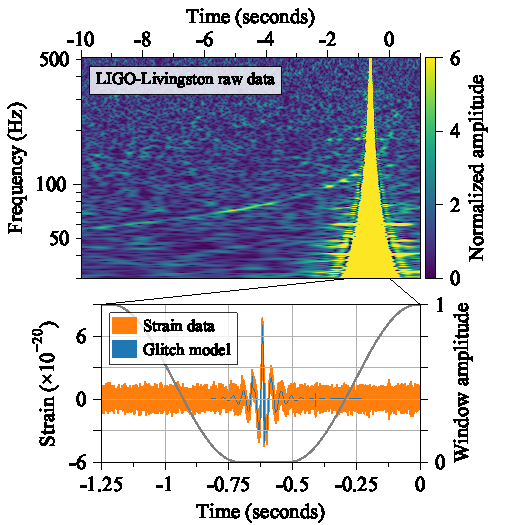
\includegraphics[width=1.0\linewidth]{images/6_earlywarning/gw170817/GW170817_glitch_subtraction.pdf}
    \caption{The Q-scan~\cite{qscan:2004} of the LIGO-Livingston data containing GW170817~\cite{GW170817:2017}, with a very loud wide bandwidth glitch present (top). The glitch was initially subtracted from the data using a windowing function to reduce the amplitude of the data containing the glitch to $0$, this windowing function can be seen as a grey line in the bottom figure. The glitch was also modelled using Bayeswave~\cite{BayesWave:2015} and subtracted from the data to preserve the \gwadj signal power found beneath the glitch, this glitch model (blue line) can be seen overlapping the strain data (orange line) in the bottom figure. This figure has been taken from~\cite{GW170817:2017}.}
    \label{6:fig:gw170817_glitch}
\end{figure}
%
In the fourth observing run we now have well tested and robust search pipelines for \gws and as previously stated, we expect a maximum latency of $20$ seconds post-merger~\cite{PyCBC_Live:2018}, glitches can be auto-gated and BAYESTAR~\cite{BAYESTAR:2016} can produce sky maps in a few seconds.

We can demonstrate the early warning search's efficacy on GW170817. Table~\ref{6:tab:gw170817_early_warning} displays the template bank cutoff frequencies alongside the network SNR of the early warning search searching for GW170817 in the original data and a GW170817-like injection in simulated data with the current detector noise curve, also shown is the time pre-merger (warning) at which GW170817 will reach the specified frequency. The single detector SNR threshold is $4.5$, giving a network SNR threshold of $6.36$. GW170817 was much louder in the LIGO-Livingston interferometer, LIGO-Hanford's single detector SNR did not increase above the threshold until the $56 \, \text{Hz}$ frequency cutoff, at which the network SNR also crossed the threshold---$12 \, \text{seconds}$ prior to the merger. The GW170817-like injection into the O4 noise curve has very large SNRs in all the frequencies, and the $29 \, \text{Hz}$ template was observed with a $67 \, \text{second}$ warning.
%
\begin{table}[ht]
    \centering
    \setlength{\tabcolsep}{4pt}
    \rowcolors{4}{white}{lightgray}
    \begin{tabular}{cccc}
        \toprule
        \multicolumn{1}{c}{\textbf{Frequency}} & \multicolumn{2}{c}{\textbf{Network SNR}} & \multicolumn{1}{c}{\textbf{Warning}} \\
        \cmidrule(lr){1-4}
        \textbf{Cutoff [Hz]} & \textbf{Original Data} & \textbf{O4 Injection} & \textbf{Time [s]} \\
        \midrule
        29 & 6.19 & 13.26 & 67 \\
        32 & 5.76 & 18.58 & 52 \\
        38 & 6.11 & 21.96 & 33 \\
        44 & 6.25 & 25.87 & 22 \\
        49 & 6.19 & 24.42 & 17 \\
        56 & 7.04 & 35.24 & 12 \\
        \bottomrule
    \end{tabular}
    \caption{The signal-to-noise ratio values for the \gwadj events with corresponding frequency cutoff found by the PyCBC Live early warning search when searching over the data which contains GW170817~\cite{GW170817:2017} (Original Data) and data which contains a GW170817-like injection into representative data from the fourth observing run (O4 Injection). Also shown is the time before merger in which the event was found (Warning Time).}
    \label{6:tab:gw170817_early_warning}
\end{table}
%
By implementing an early warning search in PyCBC Live we are capable of identifying \gwadj signals before merger. This will aid in localising potentially electromagnetically bright \gwadj signals and inform telescopes of all frequency ranges to capture as much of the electromagnetic counterpart as possible, enabling greater quality multi-messenger astronomy.


\section{\label{6:sec:injection-tests}Testing the early warning search}

The early warning search has been operating throughout the fourth observing run, and is yet to see any early warning events. A Mock Data Challenge, which cyclically re-runs $40$ days of third observing run data, is being used to test the capabilities of the early warning search and has suggested that the search is not running optimally.

To thoroughly evaluate this search pipeline's performance, we want to carry out the first large scale injection study of early warning-like \gwadj signals to directly test the efficacy of the search. By performing this injection study, we will identify any problems and improvements that can be made to enable the greatest possibility of detecting multi-messenger events via early warning in current and future observing runs.

In this section, we describe the injection study of the early warning search, detailing the parameters of the injection set used and the results of the study; the total number of injections found with at least one candidate event and the total number of candidate events found for all injections.

\subsection{\label{6:sec:injection-set}Searching for thousands of \gwadj injections}

To test the capabilities of the early warning search an injection campaign was performed, similar to the injection campaigns performed in chapters~\ref{chapter:4-archenemy} and~\ref{chapter:5-pycbc-live}. The injection parameter value ranges match the early warning template bank, therefore, the injection set used in this test contains exclusively signals that should be seen by the early warning search. The injection set contains $32,599$ unique injections placed every ${\sim}100$ seconds, encompassing $3,456,000$ seconds or exactly $40$ days worth of data. The signal parameters and value ranges can be seen in Table~\ref{6:tab:ew_inj_params}.
%
\begin{table}[ht]
    \centering
    % \small
    \setlength{\tabcolsep}{4pt}
    \rowcolors{2}{white}{lightgray}
    \begin{tabular}{ccc}
        \toprule
        \multicolumn{3}{c}{\textbf{Variable Parameters}} \\
        \cmidrule(lr){1-3}
        \textbf{Parameter} & \textbf{Value Range} & \textbf{Prior Distribution} \\
        \midrule
        Primary Mass, $m_1$ & $1.0\text{--}3.0$ [$\text{M$_{\odot}$}$] & uniform \\
        Secondary Mass, $m_2$ & $1.0\text{--}3.0$ [$\text{M$_{\odot}$}$] & uniform \\
        Primary Spin z-component, $spin1z$ & $-0.05\text{--}0.05$ & uniform \\
        Secondary Spin z-component, $spin2z$ & $-0.05\text{--}0.05$ & uniform \\
        Phase, $\phi_{c}$ & $0\text{--}2\pi$ & uniform angle \\
        Inclination, $\iota$ & $0\text{--}\pi$ & $\sin$ angle \\
        Polarisation, $\psi$ & $0\text{--}2\pi$ & uniform angle \\
        Right Ascension, $\alpha$ & $0\text{--}2\pi$ & uniform sky \\
        Declination, $\delta$ & $-\frac{\pi}{2}\text{--}\frac{\pi}{2}$ & uniform sky \\
        \bottomrule
        \multicolumn{3}{c}{\textbf{Static Parameters}} \\
        \cmidrule(lr){1-3}
        \textbf{Parameter} & \textbf{Value} & \textbf{} \\
        \midrule
        Waveform Approximant & IMRPhenomXAS~\cite{IMRPhenomXAS:2020} & \\
        Lower Frequency, $f_{lower}$ & 17 [$\text{Hz}$] & \\
        Reference Frequency, $f_{ref}$ & 17 [$\text{Hz}$] & \\
        \bottomrule
    \end{tabular}
    \caption{The parameters used to create the injection set used to test the PyCBC Live early warning search. Variable parameters will be assigned a random value within in the value range, distributed across all injections according to the prior distribution. Static parameters are the same for all injections in the injection set. Created using PyCBC~\cite{PyCBC_package:2021}.}
    \label{6:tab:ew_inj_params}
\end{table}
%

We first simulate the injections to create the injection set. The injections are then distributed uniformly in SNR between $12\text{--}60$. We then inject the injections into simulated coloured noise therefore, no non-Gaussian artefacts exist in the data.

\subsection{\label{6:sec:results}Results of the early warning injection test}

We expect injections can be seen by up to six templates corresponding to the six different frequency cutoffs. With $32,599$ injections in the injection set we could expect a maximum of $195,594$ candidate events in the results. We can expect some deviation to this number due to false events caused by random noise and the lower frequency cutoff templates not finding events for low SNR injections---some injections are just too quiet to be seen.

We create and run the early warning search on the $40$ days of data containing the injections for both LIGO-Hanford and LIGO-Livingston to find two-detector coincidences. This is consistent with the PyCBC Live early warning search which currently doesn't use Virgo data to identify candidate events. The total number of candidate events found is $175,219$, we can correlate a candidate event's time of coalescence with the known injection times to eliminate $1,211$ candidate events which were not found within a short $2 \, \text{second}$ window of an injection time of coalescence. The total number of candidate events found for all injections is $174,008$, Figure~\ref{6:fig:cand_hist_dupes} shows a histogram of the number of candidate events found per injection.
%
\begin{figure}
    \centering
    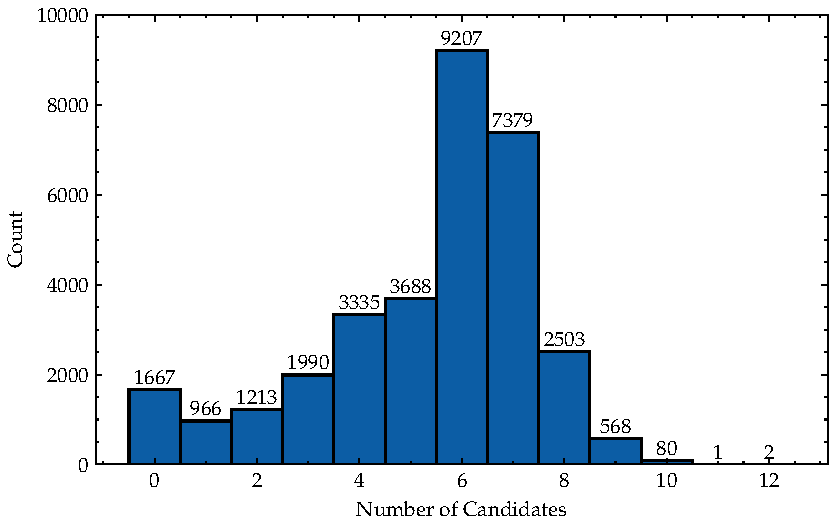
\includegraphics[width=1.0\textwidth]{images/6_earlywarning/results/count_histogram_dupes.pdf}
    \caption{A histogram showing the number of injections (Count) found with varying numbers of candidate events (Number of Candidates) by the PyCBC Live early warning search. The exact number of counts is displayed on top of the histogram bars.}
    \label{6:fig:cand_hist_dupes}
\end{figure}
%

Upon inspection of Figure~\ref{6:fig:cand_hist_dupes} we immediately identify an issue with the early warning search; the histogram shows us a large number of injections which have been found with greater than six candidate events. This is unexpected and we will explore the cause of this in the following sections, as well as other identified issues.

\section{\label{6:sec:false-problems}False events}

With these results we can evaluate the performance of the early warning search and identify the problems that we initially set out to find. For each identified problem, we describe its source, estimate the number of injections affected, and detail potential solutions to be implemented into the early warning search to prevent the problem from occurring in future observing runs. We will begin with the problem identified by Figure~\ref{6:fig:cand_hist_dupes}, where the early warning search is identifying too many candidate events for some injections.

\subsection{\label{6:sec:duplicate-frequency-cands}Finding duplicate frequency cutoff candidates}

% Lay out the problem
%  Injections seen with more than 6 events
%  Injections can only be seen with $6$ max
%  What is happening?
%  Some frequencies are seen twice
%  What?? How can that happen if the search picks the best coincidence in the second that corresponds to the final frequency truncation?

The template bank used by the early warning search contains templates for six different frequency cutoffs. The time before merger corresponding to each frequency cutoff is injection specific and it is expected that when the early warning search reaches that time, it would identify a candidate event found by a template with the correct frequency cutoff. This then places a maximum number of events found for each injection using the template bank at six events.

We have observed injections that have been seen with more than six candidate events. These candidates must have frequency cutoffs equal to one of the six found in our template bank and therefore some frequency cutoffs have been found multiple times for an injection. This should not be possible as the time before merger for the frequency cutoff would correspond to a stride in the early warning search and only the best coincident event can be chosen by the early warning search as a candidate.

\subsubsection{\label{6:sec:cands-across-bounds}Candidates straddling search boundaries}
%  Well, some truncations are close to the boundary
%  Others are across the boundary
%  There is enough lee-way to pick two in two separate seconds
%
\begin{figure}
       \centering
    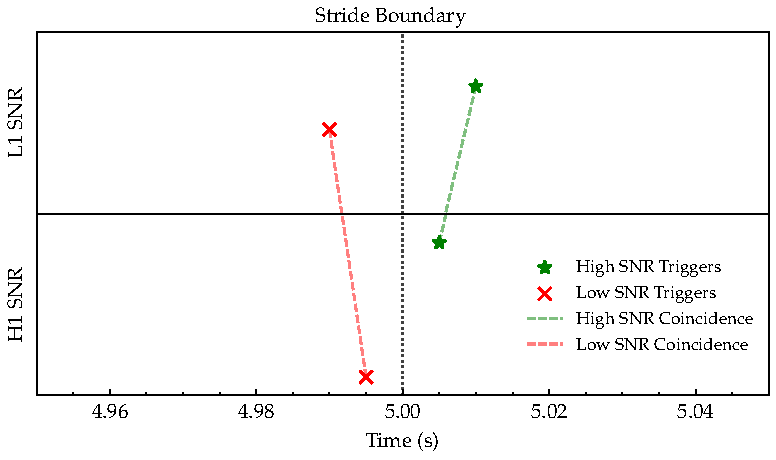
\includegraphics[width=0.75\textwidth]{images/6_earlywarning/identified-problems/cands_across_bounds.pdf}
    \caption{An illustration of two candidate events being found with the same frequency cutoff for a single injection. The red coincidence has lower single detector and coincidence SNR, but both are above SNR threshold due to the frequency cutoff template ending very close to the analysis stride boundary, this event is uploaded as a candidate event. The green coincidence is the `proper' coincidence found after the frequency cutoff template has ended and it also uploaded after the first one, leading to two events with the same frequency cutoff being uploaded for one \gwadj signal.}
    \label{6:fig:candidates_across_boundaries}
\end{figure}
%

The early warning search operates on a single second analysis stride, meaning every single second the template bank is matched filtered with the data to discover any \gwadj events. It is possible that the pre-merger time corresponding to a frequency cutoff will lie very near to the boundary between search strides. In this case, the search will record an event found in the first stride and will then again record another event in the second stride with the same frequency cutoff.

Figure~\ref{6:fig:candidates_across_boundaries} is a demonstration of this possibility. Either event can have a higher SNR when compared to the other, but the two scenarios can be treated differently to prevent some duplicate events being uploaded in the future. If the event found in the first stride has a higher SNR than the second stride we can prevent an upload of the second event (provided the template frequency cutoff is the same)---this is already done by the PyCBC Live Single Detector search~\cite{PyCBC_singles:2022}---but if the event found in the second stride has a higher SNR than the first then we will have to upload two events. We cannot delay uploading the first event.

\subsubsection{\label{6:sec:trigs-across-bounds}Triggers across search boundaries}
%  The search forces a coincidence in the first second and then finds the actual one in the second second
%
\begin{figure}
       \centering
    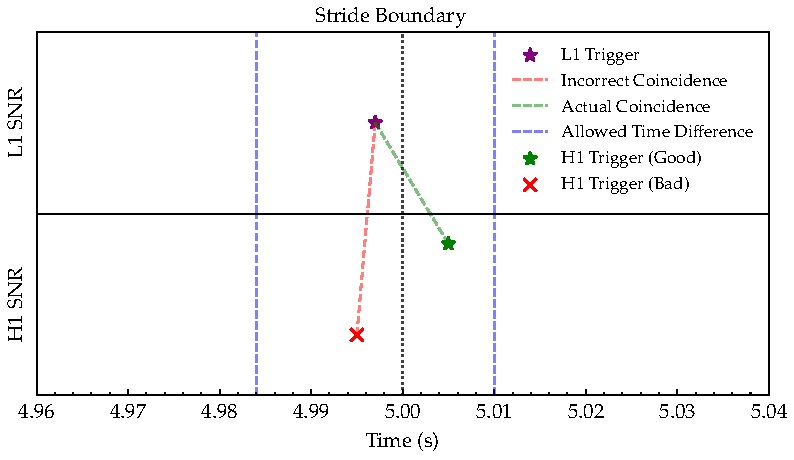
\includegraphics[width=0.8\textwidth]{images/6_earlywarning/identified-problems/trigs_across_bounds.pdf}
    \caption{An illustration of two coincident candidate events being uploaded for the same frequency cutoff. The L1 trigger for the coincidence arrives in the analysis stride and the H1 trigger arrives in the next analysis stride. The early warning search has found a low significance H1 trigger in the first analysis stride and made a low significance coincidence. When the second analysis stride is analysed the correct coincidence will be found and the same L1 trigger is uploaded again with another coincident trigger at the same frequency cutoff.}
    \label{6:fig:triggers_across_boundaries}
\end{figure}
%
The stride boundary can have another effect, which causes duplicate frequency events to be uploaded. Coincident triggers between detector 1 and detector 2 have an allowed time difference in each detector to account for the physical light-travel time of the \gw and a smaller amount of computational timing errors. It is possible for the two single detector triggers to appear across a stride boundary.

The trigger will first be seen in detector 1, which will be seen as a highly significant single detector trigger by the early warning search, where it will attempt to match with a coincident trigger in the other detector. As previously mentioned, this could be Gaussian noise which happens to match well enough for a low-significance coincidence to be made, or it could be the final point in a rising SNR time series. When detector 2 records the trigger in the next stride the early warning search will create the actual significant coincident event using the same detector 1 trigger twice. Therefore, we will get two candidate events at the same final frequency cutoff with one being less significant than the other. A demonstration of this case is seen in Figure~\ref{6:fig:triggers_across_boundaries}.

This is an unavoidable failure mode of the early warning search, we require the light travel time in the ranking statistic to form coincidences between single detector triggers and this will naturally fall across the stride boundary for some injections. 

% Example once again of the same trigger being used for both events? H1 SNR the same, L1 snr different (much lower and much higher)
% - Example
% - How often it happened
% - Impact


% Total number of injections with duplicate frequencies: 13098
% Fraction of total injections: 40.172984909827015
We find that $13,098$ injections ($40.17\%$ of the total) were found with at least one duplicate frequency and $17,432$ duplicate frequencies can be removed from our results leaving $156,576$ unique candidate events remaining. Figure~\ref{6:fig:cand_hist_dupes_removed} recreates Figure~\ref{6:fig:cand_hist_dupes} where the duplicate candidate events have not been included.
%
\begin{figure}
    \centering
    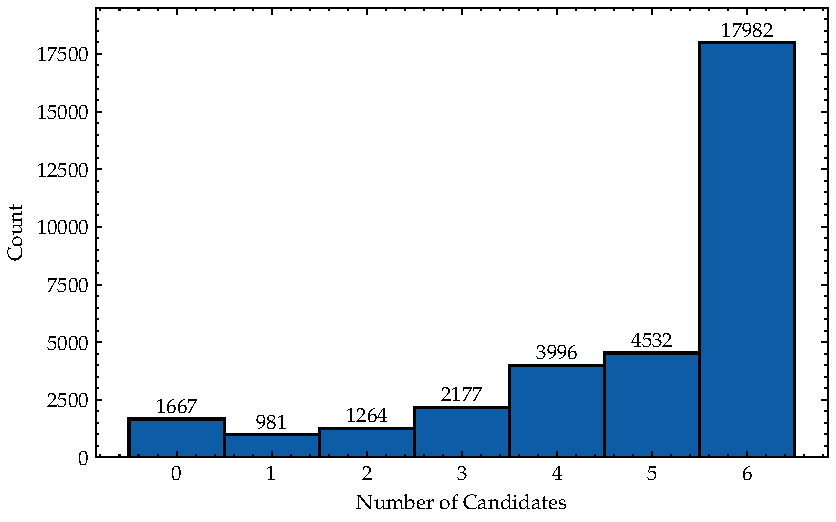
\includegraphics[width=1.0\textwidth]{images/6_earlywarning/results/count_histogram_dupes_removed.pdf}
    \caption{A histogram showing the number of injections (Count) found with varying numbers of candidate events (Number of Candidates) by the PyCBC Live early warning search. The exact number of counts is displayed on top of the histogram bars.}
    \label{6:fig:cand_hist_dupes_removed}
\end{figure}
%

Candidate events are all treated independently and while the additional events uploaded to GraceDB may be confusing, \gwadj signals on GraceDB commonly have multiple events uploaded per pipeline with multiple pipelines. Therefore, the event with the highest SNR will be preferred until a higher SNR event is identified. 

\subsection{\label{6:sec:false-alarms}Low significance candidate events}

We have discussed false alarm candidate events that do not have times of coalescence consistent with any known injection time of coalescence and have removed $1,211$ candidates from our final results. There is a possibility of a false alarm candidate event to have a time of coalescence that falls nearby to an injection. These are easy to identify because those that appear at a lower frequency will not have the corresponding candidates from the next frequencies in the template bank. This is not something the early warning search can take into account in low-latency, but it is something that can be used post-detection to confirm the legitimacy of an event.
%
\begin{figure}
       \centering
    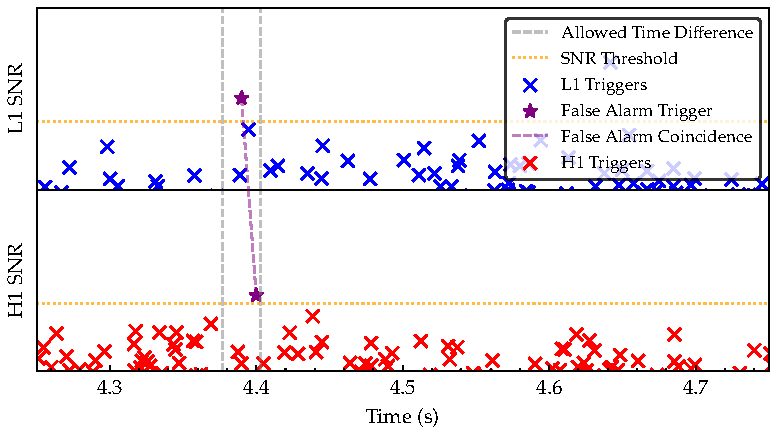
\includegraphics[width=\textwidth]{images/6_earlywarning/identified-problems/low_sig_cands.pdf}
    \caption{An illustration of a coincident candidate being found by the alignment of Gaussian noise triggers in two detectors. The crosses represent the single detector triggers identified by the \gwadj search, triggers found above the SNR threshold can be considered a single detector trigger. Coincident triggers have to lie inside the allowed coincidence window, shows by the grey dashed lines around the L1 trigger.}
    \label{6:fig:low_significance_candidates}
\end{figure}
%
The injection set used in this search was made using a PSD representative of the advanced LIGO noise curve~\cite{aLIGO_design_curve:2018} and therefore is coloured Gaussian noise, not containing any non-Gaussian noise transients. This means that when we identify a false-alarm candidate it has been caused by Gaussian noise triggers aligning in between the two detectors and finding a coincidence, a demonstration of this can be seen in Figure~\ref{6:fig:low_significance_candidates}.

We can identify further false-alarm candidate events in two ways: look for injections with single candidates that have frequency cutoffs not equal to the highest cutoff in the template bank ($56 \, \text{Hz}$); and by comparing the injection template and the candidate event template. We observed $99$ injections with single candidates and a further $39$ candidate events with a mismatch between template $\mathcal{M}$ and injection $\mathcal{M}$ of ${\pm}1\%$.

Of the original $174,088$ candidate events identified and we have been able to eliminate $17,570$ candidate events that were caused by boundary issues or false-alarms, leaving $156,438$ candidate events identified by the early warning search during the injection study. Figure~\ref{6:fig:cand_hist_all_removed} shows the distribution of the number of candidate events found per injection, where $13,225$ injections have additional unexpected candidate events.
%
\begin{figure}
    \centering
    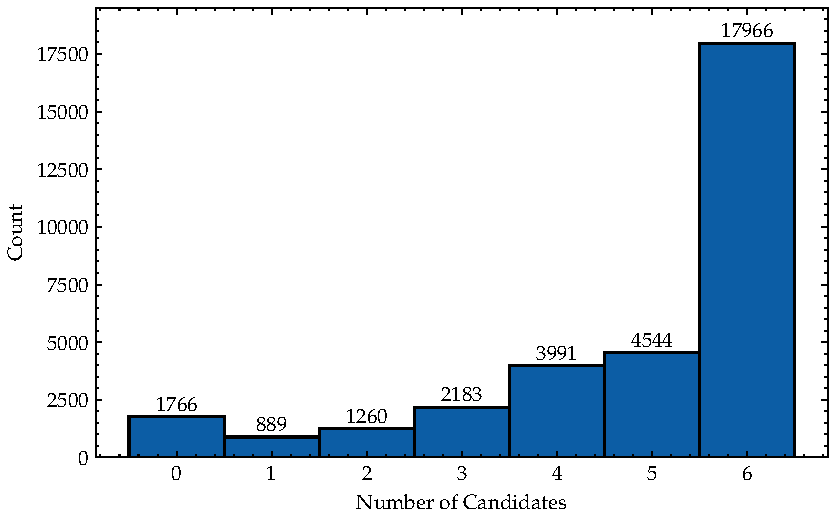
\includegraphics[width=1.0\linewidth]{images/6_earlywarning/results/count_histogram_all_removed.pdf}
    \caption{A histogram showing the number of injections (Count) found with varying numbers of candidate events (Number of Candidates) by the PyCBC Live early warning search. The exact number of counts is displayed on top of the histogram bars.}
    \label{6:fig:cand_hist_all_removed}
\end{figure}

\section{\label{6:sec:outside-coinc-window}Candidate events we did not see}

% What is the broad problem?    
% What are some ways it manifests
% How can we solve this problem
%  Coinc Window - Fairhurst
%  PhaseTD tuning for statistic
%  Sample rate issue

We have identified injections that have seen extra candidate events from what we expect and now we can look at injections where we expected to see more events than we did. We count the number of candidate events for each injection and compare to the expected number of candidate events considering the lowest frequency cutoff the injection was found with. For example, if an injection has been seen at $29 \, \text{Hz}$ then we would expect six candidate events in total, whereas for an injection seen first at $49 \, \text{Hz}$ we would only expect two candidate events ($49 \, \text{Hz}$ and $56 \, \text{Hz}$). A further inspection of these candidate event SNRs can reveal another issue with the observations, we expect a monotonic increase in the SNR of each subsequent frequency cutoff in the template bank. If the SNR between consecutive candidates does not exhibit this SNR increase then we know this injection has encountered a problem we must investigate. Figure~\ref{6:fig:non-monotonic-snr} shows an illustration of these injections, where the 
$32 \, \text{Hz}$ has either not been seen at all or has been seen with a much lower SNR than what is expected.

\begin{figure}
       \centering
    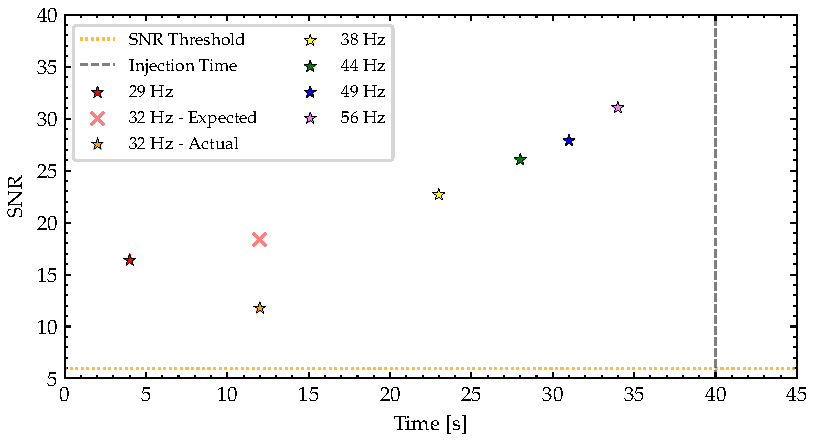
\includegraphics[width=\textwidth]{images/6_earlywarning/identified-problems/non_mono_snr.pdf}
    \caption{An illustration of the expected and SNRs for the case where one of the event's coincident triggers have fallen outside the coincident timing window. In the first case we see a missing frequency in the SNR evolution (indicated by the red cross), in the second case we see a non-monotonic increase in SNR where the search has found a low significance event to `fill' the gap (shown by the orange star).}
    \label{6:fig:non-monotonic-snr}
\end{figure}

\subsection{\label{6:sec:light-travel-time}Coincident triggers outside the light travel time}

We investigate the frequency of the missing candidate events for injections that have a gap in frequency evolution and obtain the following counts per frequency cutoff: $29 \, \text{Hz} = 0$ (We do not distinguished between missed and not found for the first frequency cutoff), $32 \, \text{Hz} = 288$, $38 \, \text{Hz} = 162$, $44 \, \text{Hz} = 132$, $49 \, \text{Hz} = 168$, $56 \, \text{Hz} = 140$. Some injections have multiple missing frequencies, and in total we find $873$ injections ($2.68\%$) are missing at least one expected candidate event in its frequency evolution. This is a lower limit on the true number of injections with missing candidate events, we are unable to count injection where: the $56 \, \text{Hz}$ template was the only one above the SNR threshold and was missed; the missed frequency is the lowest frequency in the evolution, for example $29 \, \text{Hz}$, then we are just assuming that the $29 \, \text{Hz}$ did not have enough SNR to be seen and wasn't `missed' in this context.

The early warning search will output all the triggers found when matched filtering the template bank and the data every second. Candidate events are detected in the analysis segment containing the end time of the template, which represents the frequency cutoff for the injection. Therefore, we can look at the triggers found by the search to determine why a candidate event was not identified. The injections with missing frequencies all record single detector triggers above the SNR threshold and with the best matching template for both detectors but, we have identified that the time difference between these two triggers is greater than our allowed coincidence timing window---a component of the coincident ranking statistic to demand physical time differences between triggers.

The two LIGO detectors are separated by a straight line through the Earth $3002$ kilometres long. Given the speed of light there is a $0.01 \, \text{second}$ window for the \gwadj signal to travel from one detector to the other. We allow a further $0.003 \, \text{seconds}$ in addition to the light travel time to account for any detection response, timing, or waveform uncertainties. This give a total allowed coincidence timing window of $0.013 \, \text{seconds}$. An illustration of this problem can be seen in Figure~\ref{6:fig:outside_coinc_window}. How is it possible for our `coincident' triggers from our injection set to lie outside the allowed coincidence timing window?
%
\begin{figure}
    \centering
    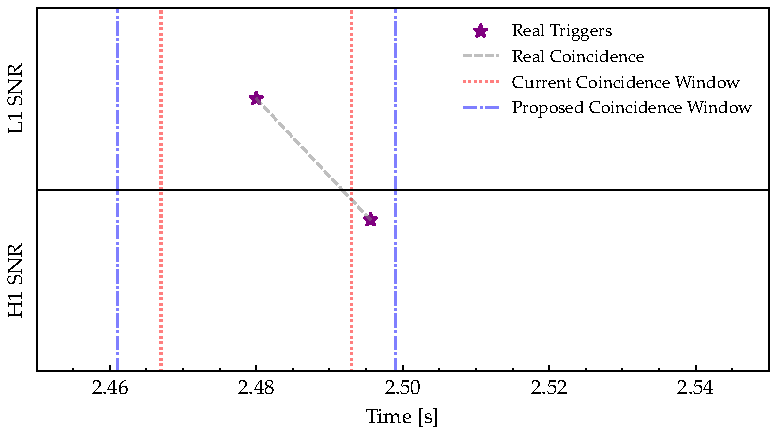
\includegraphics[width=\textwidth]{images/6_earlywarning/identified-problems/outside_coinc_window.pdf}
    \caption{An illustration of two single detector triggers being found outside the allowed coincidence time difference window. The current coincidence window shows the triggers falling outside the window and therefore the search does not form a coincidence. With the new proposed coincidence time window the coincidence would be found.}
    \label{6:fig:outside_coinc_window}
\end{figure}
%

\subsubsection{\label{6:sec:timing_error}Timing accuracy error}

As described in~\cite{Fairhurst:2010}, the accuracy of the candidate time in a detector can be determined by,
%
\begin{equation}
    \sigma_{t} = \frac{1}{2\pi\rho\sigma_{f}}
    \label{6:eqn:timing_acurracy}
\end{equation}
%
where the timing accuracy, $\sigma_{t}$, is inversely proportional to the SNR, $\rho$, and the effective bandwidth of the source, $\sigma_{f}$ which is defined as
%
\begin{equation}
    \sigma_{f}^2 = \left(\int^{\infty}_{0} df \frac{f^{2}|\hat{h}(f)|^{2}}{S(f)}\right) - \left( \int^{\infty}_{0} df \frac{f|\hat{h}(f)|^{2}}{S(f)}\right)^{2} .
    \label{6:eqn:eff_bandiwdth}
\end{equation}
%
where the waveform $\hat{h}$ is normalised such that $\int \frac{|\hat{h}(f)|^{2}}{S(f)}df = 1$. We use the same PSD to normalise that has been used throughout the injection study. As shown in Table 1. of~\cite{Fairhurst:2010}, the timing error for a binary neutron star system in an advanced LIGO configuration with a BNS range of $160 \, \text{Mpc}$ is $0.46 \, \text{ms}$. This is negligible when compared to our light-travel time of $10 \, \text{ms}$. We can approximately calculate the timing accuracy of the early warning templates using equations~\ref{6:eqn:timing_acurracy} and~\ref{6:eqn:eff_bandiwdth}, where the \gwadj strain term, $|h(f)|$, is assumed to be equal to the inspiral frequency evolution of a binary neutron star signal, $f^{-\frac{7}{6}}$. The estimated effective bandwidths and timing accuracy errors can be seen in Table~\ref{6:tab:timing_errors}.
%
\begin{table}[ht]
    \centering
    \setlength{\tabcolsep}{4pt}
    \rowcolors{3}{white}{lightgray}
    \begin{tabular}{ccc}
        \toprule
        \textbf{Frequency [Hz]} & $\sigma_{f}$ [Hz] & $\sigma_{t}$ [ms] \\
        \midrule
        29 & 3.38 & 5.89 \\
        32 & 4.19 & 4.75 \\
        38 & 5.79 & 3.44 \\
        44 & 7.37 & 2.70 \\
        49 & 8.68 & 2.29 \\
        56 & 10.51 & 1.89 \\
        1024 & 90.05 & 0.22 \\
        \bottomrule
    \end{tabular}
    \caption{The effective bandwidth, $\sigma_{f}$, and timing accuracy error, $\sigma_{t}$, for the frequency cutoffs (Frequency) found in the early warning template bank as well as the full bandwidth frequency ($1024 \, \text{Hz}$).}
    \label{6:tab:timing_errors}
\end{table}
%
Using an SNR of $8$ (and a lower frequency of $17$ Hz) yields $1$ sigma timing errors from $5.89$ to $1.89$ milliseconds for the early warning frequency cutoffs, where higher frequencies have smaller timing errors. The current allowed error is $3 \, \text{ms}$ therefore we can expect to miss candidates from all the frequency cutoff templates when the timing error places coincident triggers outside the current allowed coincidence time window. This can be remedied with a widening of the window which could be done on a template dependent basis, with a timing accuracy error dependent on the frequency cutoff.

The PyCBC Live early warning search uses a sample rate of $256 \, \text{Hz}$ which contributes to a worse timing accuracy. The time between samples is $3.9 \, \text{ms}$ and a trigger found by another detector $3$ samples later will be within the allowed window of $13 \, \text{ms}$ but being $4$ samples later equals a time difference of $15.6  \, \text{ms}$; falling outside the window. We can perform a subsample interpolation between samples to recover the correct trigger time within the allowed window.

\subsubsection{\label{6:sec:ew_phasetd}Early warning tuned Phase-Time-Amplitude histogram}
% Great, we've made the window bigger
% What? It still won't work? Why not?
% PhaseTD File
%  What is it?
%  How is it made?
%  How is it tuned?
%  Does it take into account time windows outside the 13ms? (no)
\begin{figure}
    \centering
    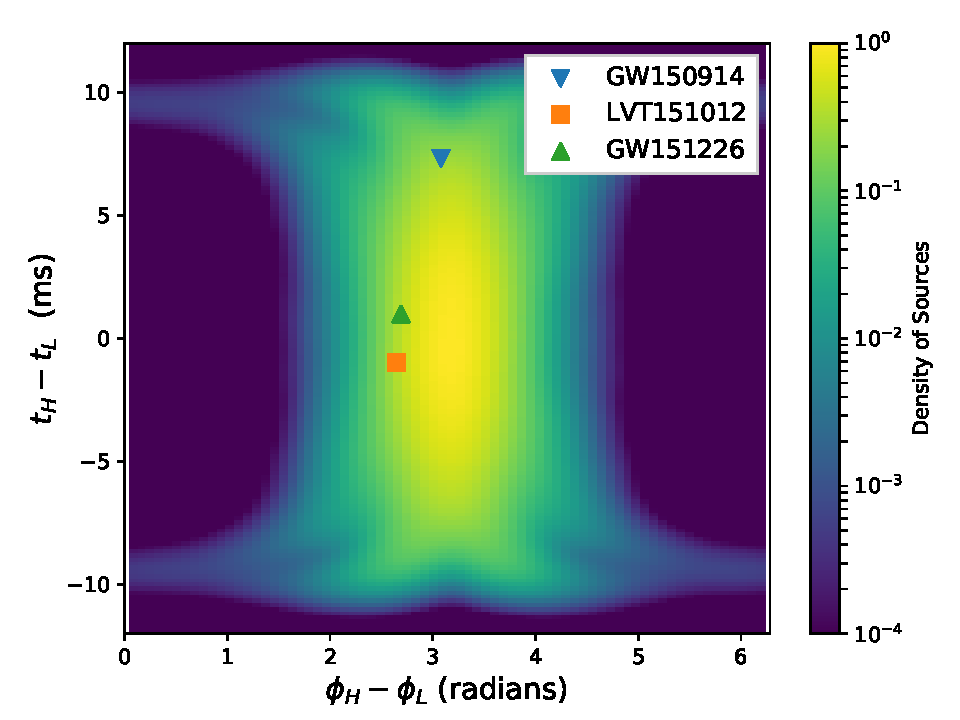
\includegraphics[width=1.0\linewidth]{images/6_earlywarning/identified-problems/phase_time.pdf}
    \caption{Phase-Time-Amplitude histogram for the PyCBC ranking statistic, showing the density of \gwadj candidate sources as a function of time delay on the y-axis, $t_H - t_L$ in milliseconds, and phase difference on the x-axis, $\phi_H - \phi_L$ in radians, between detectors. The first three \gwadj candidates have been highlighted on the plot~\cite{gwtc1:2019}. The colour scale indicates the density of sources in logarithmic scale. The histogram can be used to determine how likely a signal is based on the differences in phase, time, and amplitude recorded by each detector. Taken from~\cite{PyCBC:2017}.}
    \label{6:fig:phase-time-histogram}
\end{figure}
%
Increasing the allowed coincidence time window allows the early warning search to form coincident triggers which share the same template parameters and are physically possible (when accounting for timing accuracy error). However, we will face another problem where the coincident ranking statistic used by the early warning search will consider these events to have a very low signal rate. The coincident ranking statistic used by the early warning search is \texttt{phasetd} (phase-time delay) and is used to assess the coincidence likelihood between two triggers from different detectors.

For a two detector coincidence, the likelihood value is found by sampling from a pre-created \texttt{phasetd} 3-dimensional histogram in amplitude, time, and phase space. The file is created by simulating \gwadj signals from an isotropic distribution of sources, where each signal is assigned a random sky location (right ascension and declination), inclination and polarisation. The detector responses to the signal are calculated, from which we get the amplitudes, time, and phases for each injection in each detector. For a pair of detectors, the time difference, phase difference and relative signal amplitude are then binned into discrete bins which represent different combinations of amplitude, time, and phase difference. An example of the phase-time histogram (marginalised over amplitude) can be seen in Figure~\ref{6:fig:phase-time-histogram}~\cite{PyCBC:2017} where the density of sources at time differences greater or less than $13 \, \text{ms}$ is extremely low. Therefore, when we sample from the histogram with large time difference, we will receive very low value of the signal rate. The timing accuracy error will need to be taken account explicitly in the time difference on both trigger times.

Another improvement that can be made in the generation of the \texttt{phasetd} statistic files is including the sample rate of the search as a parameter. For a Monte Carlo simulation, the trigger time differences are as accurate as a \texttt{float64} parameter can be. Whereas the timing difference between triggers in the PyCBC Live search will only take discrete values of the time difference dependent on the sample rate, for example, the early warning search has a sample rate of $256 \, \text{Hz}$ and therefore the time difference between samples is approximately $3.9$ milliseconds. Therefore, our \texttt{phasetd} file will only ever been sampled from using time difference that are $n$-multiples of this time between samples. We can create \texttt{phasetd} files with bins in the time difference parameter space which represent the sample rate of the search and therefore can be sampled more accurately.

\subsubsection{\label{6:sec:missing-cands}Missing candidates}

We know now the search will produce triggers that fall outside the allowed coincidence timing window and fail to form a coincident event. Figure~\ref{6:fig:missing-freq-eg} shows an example of an injection which has been found with all but $1$ final frequency cutoff template. 
%
\begin{figure}
    \centering
    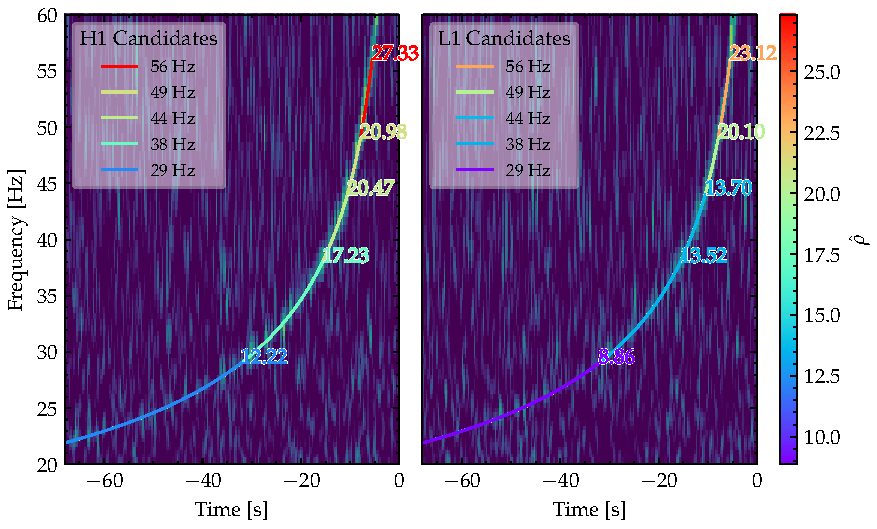
\includegraphics[width=1.0\linewidth]{images/6_earlywarning/stories/missing_freqs_example.pdf}
    \caption{An example of a \gwadj injection seen by the PyCBC Live early warning search with a missing template with frequency cutoff $32 \, \text{Hz}$.}
    \label{6:fig:missing-freq-eg}
\end{figure}
%
To verify the time difference problem, we investigated the expected network SNRs for this injection at each final frequency cutoff in both a noiseless and expected noise regime (not performed using the PyCBC Live search). The values for these can be seen in Table~\ref{6:tab:noise_snrs}.
%
\begin{table}[ht]
    \centering
    \setlength{\tabcolsep}{4pt}
    \rowcolors{2}{white}{lightgray}
    \begin{tabular}{ccc}
        \toprule
        \textbf{Frequency Cutoff [Hz]} & \textbf{Noiseless SNR} & \textbf{Noisy SNR} \\
        \midrule
        29 & 16.43 & 15.38 \\
        32 & 19.16 & 17.95 \\
        38 & 24.00 & 21.50 \\
        44 & 28.11 & 25.26 \\
        49 & 31.04 & 27.94 \\
        56 & 34.48 & 29.02 \\
        \bottomrule
    \end{tabular}
    \caption{The expected signal-to-noise ratios in both noiseless and noisy data for the \gwadj injection shown in Figure~\ref{6:fig:missing-freq-eg}. The noiseless SNR has been calculated by taking the un-normalised matched-filter of the template with itself~\cite{Brown_Thesis:2004}. The noisy SNR has been calculated by matched-filtering the template with the injection that has been injected into simulated \gwadj data.}
    \label{6:tab:noise_snrs}
\end{table}
%
We can clearly see that we are expecting to see a large network SNR for the $32 \, \text{Hz}$ template, which isn't recovered by the search. Next we are able to re-run the early warning search using a template which perfectly describes the injection parameters and in this case we still fail to recover the candidate event but, we can look into the trigger files to identify the single trigger found by both searches with the same template above the SNR threshold. We find a H1 trigger with SNR $14.55$ and an L1 trigger with SNR $12.38$ (giving a network SNR of $19.11$) and when the time difference between triggers is calculated we get $15.625 \, \text{ms}$, greater than the currently allowed $13 \, \text{ms}$. 

We then perform another search with a sample rate of $2048 \,\text{Hz}$, which doesn't find a coincidence but has a smaller time difference of $14.6 \, \text{ms}$ (still outside the window) proving that the time accuracy error is playing a part and it isn't simply a sampling inaccuracy. When performing a final search in which we expand the allowed coincidence timing window by an additional $10 \, \text{ms}$ (this can be tuned in the future) we successfully recover all $6$ events for this injection.

% However, we still need to investigate how the \texttt{phasetd} ranking statistic has responded to the highly unlikely time difference. We calculate the signal rate using
% %
% \begin{equation}
%     \log(r_s) = \frac{R - \hat{\rho}_{H}^{2} + \hat{\rho}_{L}^2}{2}
% \end{equation}
% %
% where R is the event's ranking statistic value and $\hat{\rho}_{H}$ and $\hat{\rho}_{L}$ are the single detector new SNRs. We recover a signal rate using the same \texttt{phasetd} histogram being used by the PyCBC Live search of $-24.70$. This is extremely low and therefore the signal is being considered as extremely unlikely but, the SNRs of the signal are so high such that this is compensated for and the ranking statistic value found by the search overall is around $17.77$, quite significant. This points to issues surrounding the \texttt{phasetd} histogram file that still needs to be fixed.

\subsubsection{\label{6:sec:non-mono-snr}Non-monotonic SNR evolution}
% - Example
% - How often it happened
% - Impact

Another manifestation of the timing accuracy error is the possibility for the missing frequency to be found but with a SNR not following a monotonic SNR increase across the entire injection event timeline. A demonstration of this can be seen in Figure~\ref{6:fig:non-monotonic-snr} and an example of this happening for an injection in our early warning search can be seen in Figure~\ref{6:fig:non_mono_eg}.
%
\begin{figure}
    \centering
    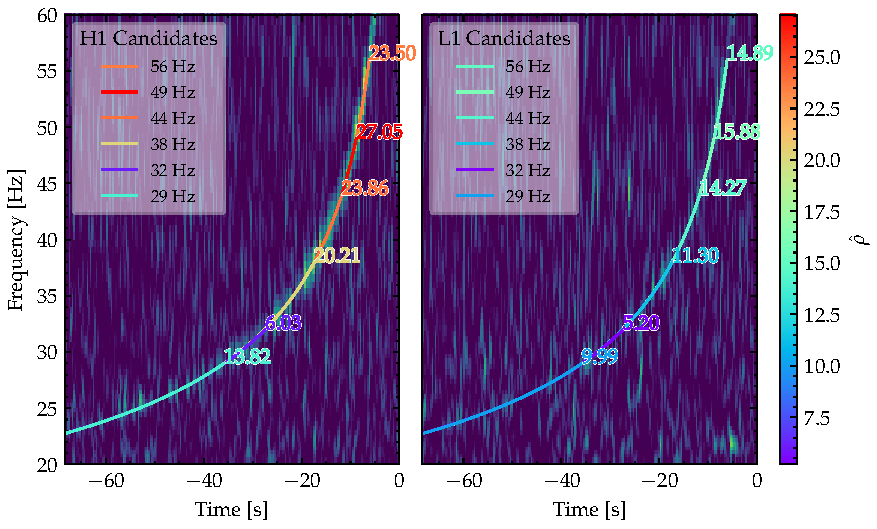
\includegraphics[width=1.0\linewidth]{images/6_earlywarning/stories/non_mono_example.pdf}
    \caption{An example of a \gwadj injection that has been found with a non-monotonically increasing signal-to-noise ratio between successive frequency cutoffs. The $32 \, \text{Hz}$ frequency cutoff \gwadj template has been seen with a lower SNR in the H1 and L1 single detector searches than the $29 \, \text{Hz}$ frequency cutoff template. This is caused by the actual $32 \, \text{Hz}$ template coincident triggers being found outside the allowed coincidence timing window.}
    \label{6:fig:non_mono_eg}
\end{figure}

It can be seen that the $32 \, \text{Hz}$ has been found by the search for this injection, but with a much lower SNR than expected and not following the monotonic SNR increase that we would expect. When investigating the triggers found we can see that the search has managed to find a low-significance trigger within the coincidence time window and has managed to form a coincidence with low SNR, similar to the low significance candidates described in Section~\ref{6:sec:false-alarms} but where one trigger is actually real. Looking into the single detector trigger files we can once again find the coincident trigger pair that should've been made if the coincidence timing window was larger and when running the search over this injection with the larger coincidence time window we find all $6$ events for this injection with the expected SNR.

We find that $997$ injections had non-monotonically increasing SNR between all successive frequency cutoffs. However, we expect a number of injections to have non-monotonically increasing SNRs due to Gaussian noise in the detector influencing the SNR values recovered for some templates. Therefore, we only count injections in which the drop between successive SNRs is greater than $5\%$ of the previous frequency cutoff template's SNR. When applying this limit, we obtain only $120$ injections with non-monotonically increasing SNR ($0.37\%$).

% Total number of injections with non-monotonic SNRs: 997
% Fraction of total injections: 3.0579070052754265
% Total number of injections with non-monotonic SNRs above threshold: 120
% Fraction of total injections: 0.368052999631947

\section{\label{6:sec:conclusion}Conclusion}

We injected $32,599$ simulated \gwadj signals into $40$ days of simulated \gwadj data and searched through this data using the PyCBC Live early warning search. The PyCBC Live early warning search found $175,219$ candidate events, $174,008$ of these candidate events can be associated with an injection in our injection set and after removing extra unexpected candidate events from duplicate frequency events and false-alarms we obtain $156,438$ candidate events for all injections.

The more significant problem identified by this injection study is the missed events that we should've seen but were didn't due to the inadequate allowed coincidence timing window between coincident triggers. We identify $873$ injections that were missing at least one expected candidate event and $120$ more which missed the coincident event but found a far less significant coincidence with a significant deviation from the expected monotonic SNR increase. In total, we missed $1,766$ injections completely however, of these we have been unable to estimate those missed due to the coincidence timing window.

To prevent \gwadj signals from being missed by the PyCBC Live early warning search a configuration change is needed to increase this window alongside an improved phase-time-amplitude histogram which accounts for coincident \gwadj triggers at these extended time differences. 

In conclusion, the early warning search is more than capable of observing \gwadj signals tens of seconds prior to the merger of the \gwadj event. We are able to disseminate information about this event to the international scientific community however, a statistic change is required in the current and future observing runs to enable the identification of \gwadj signals with time differences between detectors outside the current allowed coincidence timing window. While the early warning search is more than capable of observing these events, electromagnetically bright events have proven to be exceedingly rare and therefore we do not expect to observe an early warning event in the near future. Additionally, the early warning search is robust in its capability to detect up to five individual candidate events per \gwadj event therefore, if we miss a single one of these due to timing differences then there is a still a high likelihood of observing the \gwadj event in early warning via the other four frequency cutoffs.
